\chapter{Conclusions} \label{chap:conclusion}

\section{Discussion} \label{sec:discussion}

A framework to combine tracking and optical flow methods to improve 
object based dense motion description is presented. The pipeline is 
composed of three main steps, object tracking, segmentation and 
flow estimation. For the segmentation step a new promising video object 
segmentation algorithm was proposed, and, to the best of our knowledge, 
the introduced superpixel flow is the first energy based algorithm for superpixel matching.
This superpixel matching technique is used to track regions that belong to the background of the 
scene and allows a fine initialization of segmentation techniques, leading to a precise and stable 
segmentation method for objects in video sequences.
For the last step, a flow estimation method based on a modification of the simple-flow method to use 
the obtained segmentation mask is presented. 

The experiments showed that this object based flow estimation improves the dense motion 
estimation in comparison to optical flow techniques. This is done, of course, at the expense of involving a manually 
initialized object tracker in the process. An object detector can be added at the beginning of the pipeline, but this kind of adding would only 
worth for very specific tasks. Moreover, it is also shown than a simple 
mixing of tracking and locally computed optical flow is already better than global optical flow methods. 
This mixture seems to be in contradiction with the classic aperture problem. However, as the results are evaluated only inside an interest region (the object), this problem disappears. Thus, as the tracker provides 
a global motion displacement, and the dense flow is only computed within the given tracker windows, a 
more precise flow is obtained.


Future work can be further explored in the use of the object flow as feedback hint for tracking-by-detection methods. Also, 
several kind of applications of the object flow can be more deeply approached. For instance, 
in the structure-from-motion pipeline, video based rendering, automatic video edition, and video in-painting  among others.
Moreover, it is worth to generalize the concept of object flow to create a precise (global) optical flow method. One idea to accomplish 
this is, for instance, to over-segment the two involved frames, and initialize simple trackers to solve for the global motion of every segment, and 
then apply a heavily regularized flow estimation for every pair of segmented objects in the sequence.

\section{Final remarks} \label{sec:remarks}

   \begin{figure}[thpb]
      \centering
      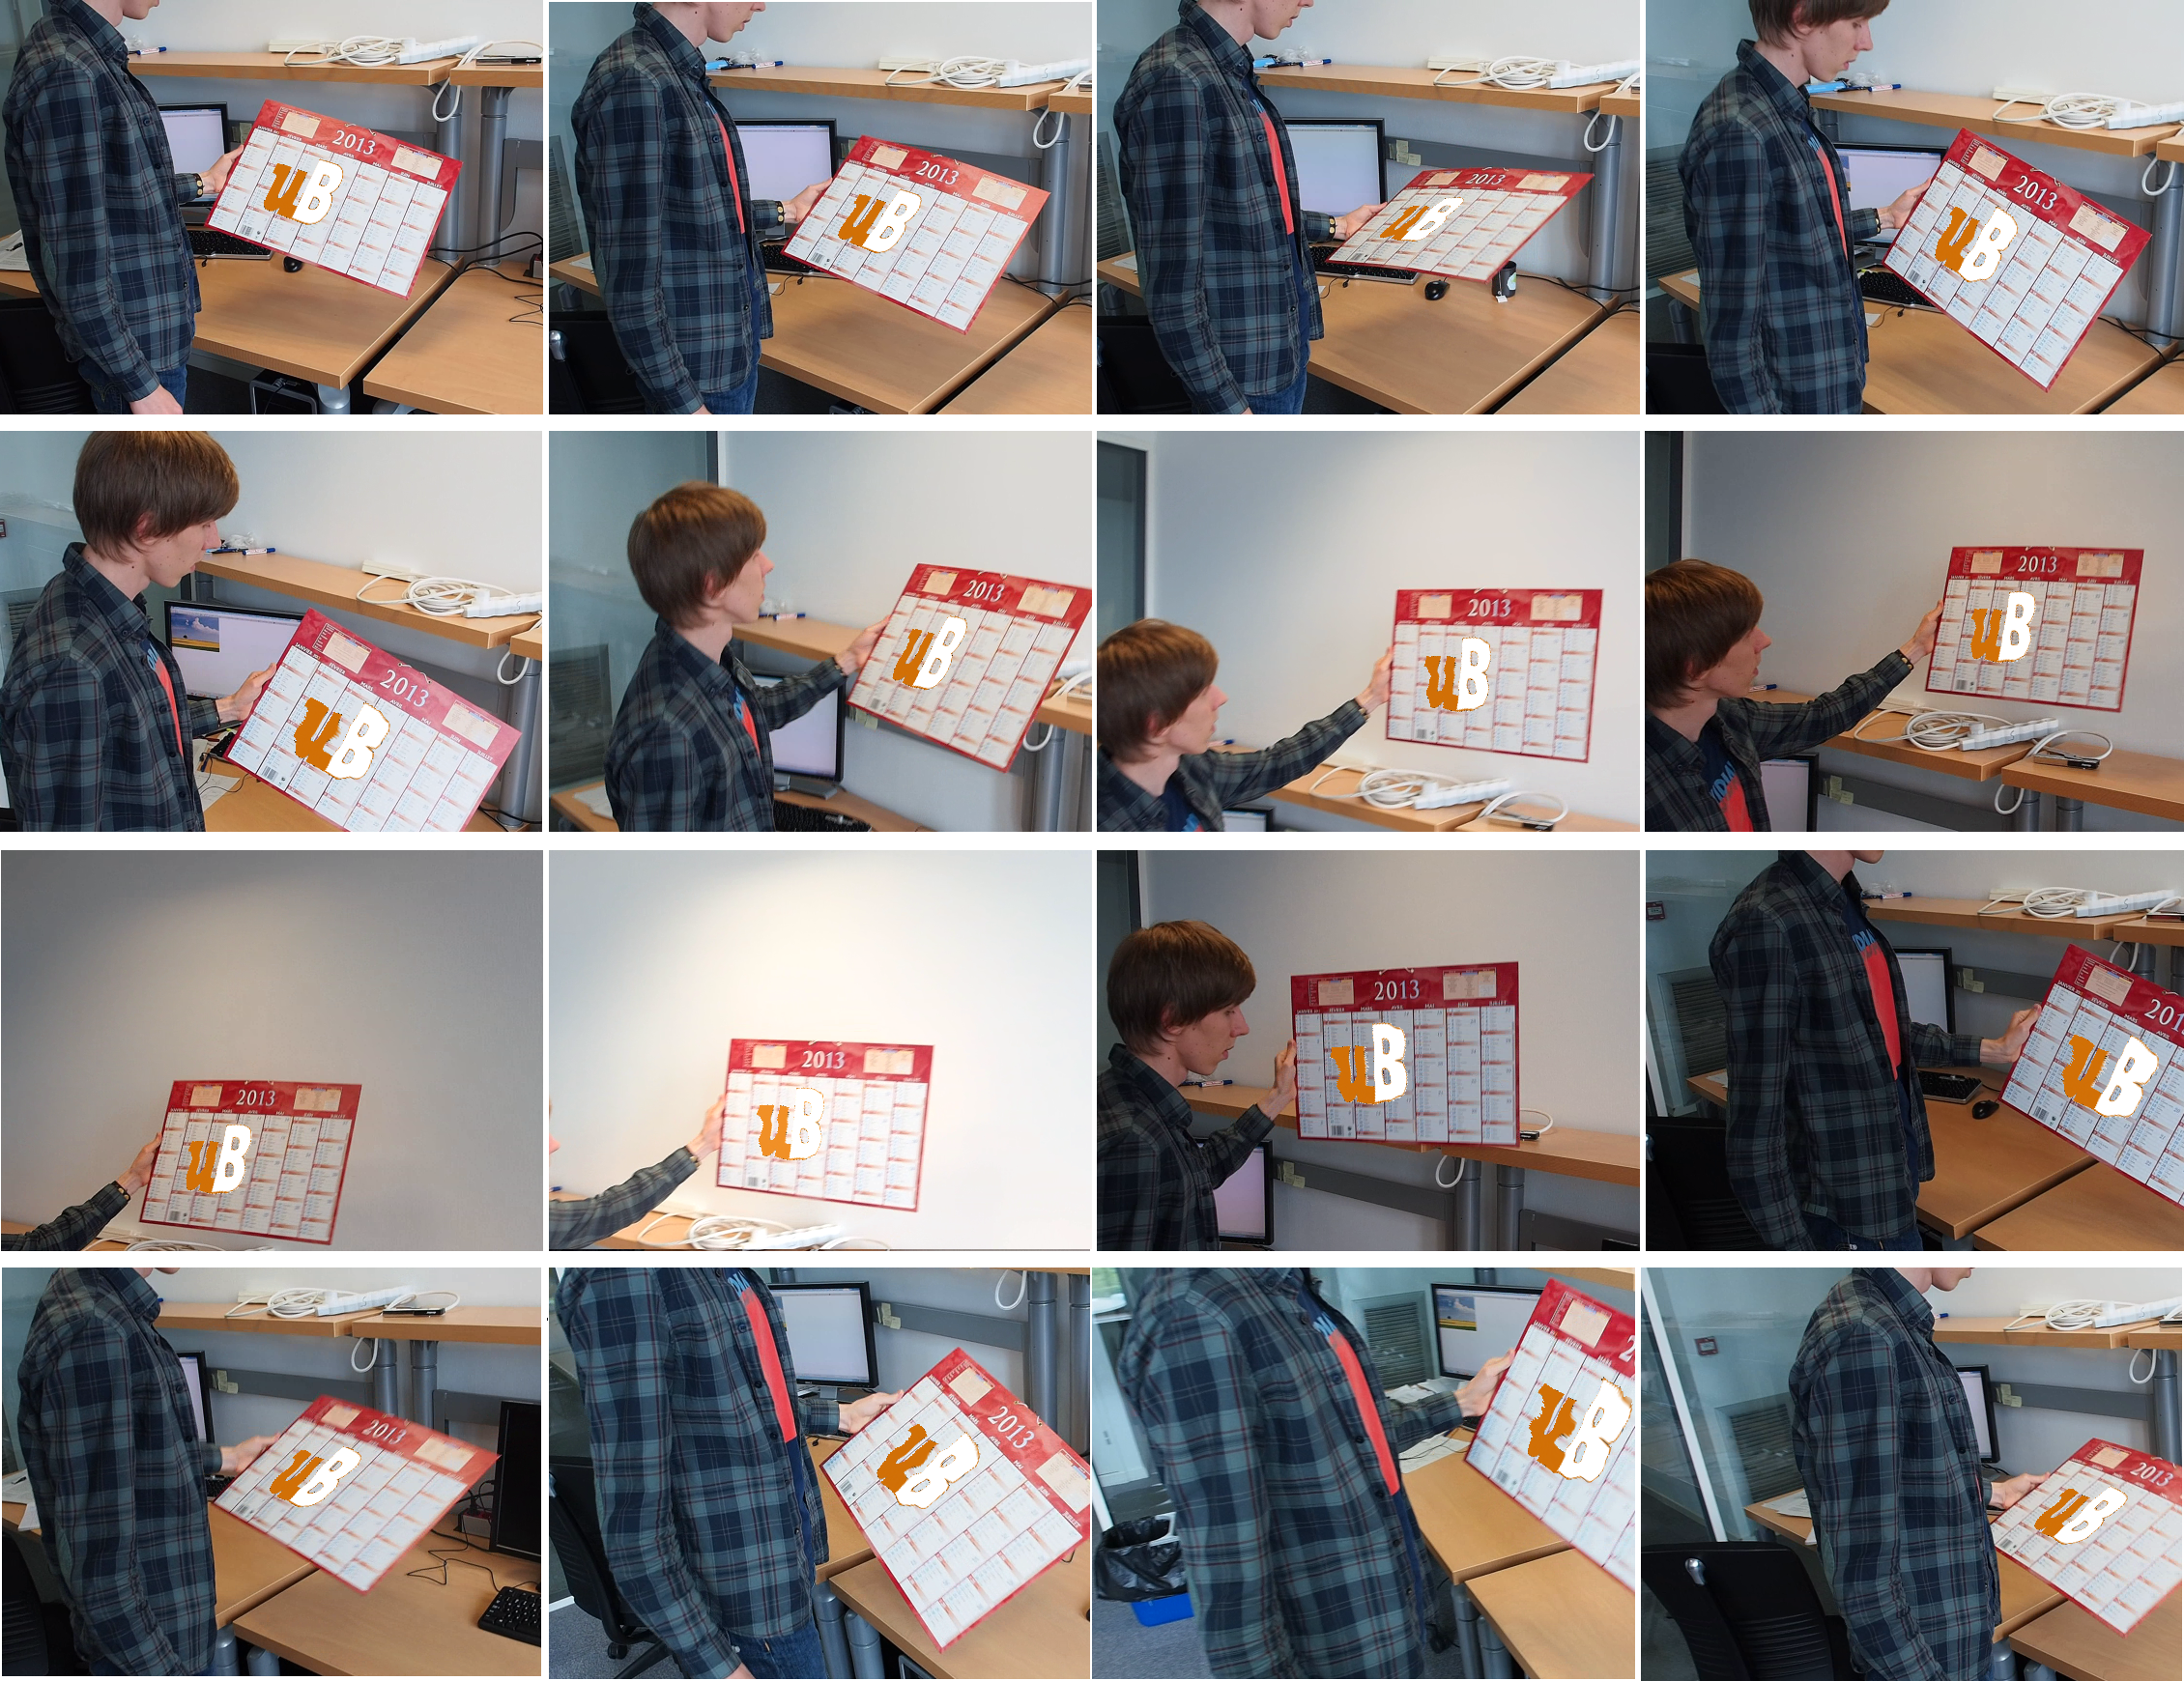
\includegraphics[width=1.00\textwidth]{../images/errors.png}
      \caption{ Sequence with different difficult cases for flow estimation methods: Autobalanace, illumination changes, specularities. }
      \label{of_errors}
   \end{figure}

\textbf{Known weaknesses}. A few remarks have to be disclosed about the object flow. As it was presented, it is also tied to the same drawbacks as the normal optical flow methods. 
For instance, the Fig. \ref{of_errors} shows how the object flow based video edition is affected by common problems related to videos: 
automatic white balance of the camera, illumination changes and specular reflections. The Fig. \ref{zoom_errors} shows a close-up to the generated 
artefacts in some of the frames. This means, for some kind of videos, for the object flow to behave accurately, some pre-processing would be needed. 
Nevertheless, as it was shown before, the object flow stands accurate when these problems are not very strong.

   \begin{figure}[thpb]
      \centering
      \includegraphics[width=1.00\textwidth]{../images/zoomerrors.png}
      \caption{Close-up to the generated artifacts due to the illumination changes and specular reflections. }
      \label{zoom_errors}
   \end{figure}

In addition, as it was shown in the Fig. \ref{sample}, the assumption of strong spatial smoothness within the object boundaries seem to affect the results 
for articulated objects. A piecewise smoothing prior can be used in a superpixelated object to minimize these kind of artifacts. This, however, was not tested.

\textbf{Other results}. The background tracking device through the superpixel flow as method 
for object segmentation in video and to enhance object tracking is under a pending patent.
The object flow pipeline, and the results obtained from the experiments 
presented in this work are summarized in a paper to be submitted to an international conference. 
A demo application for augmented reality is under development, and to the moment of 
the writing of the final draft of this document, 13.922 lines of code 
were written (11.564 in {\it .cpp} files, 
1.192 in {\it .hpp} files, and 1.166 in {\it .h} files).

